\ifanon
% \documentclass[nocopyrightspace,natbib,onecolumn,9pt]{sigplanconf}

% \newif\ifdraft\draftfalse  %% set to false in final version

% \usepackage{xspace,pads,amsmath,math-cmds,
%             math-envs,inference-rules,times,
%             verbatim,alltt,multicol,proof,url}
% \usepackage{epsfig}
% \usepackage{code} 
% \usepackage{color}
% \usepackage{tikz}

% \begin{document}
% \newcommand{\cut}[1]{}
\newcommand{\reminder}[1]{{\it #1 }}
\newcommand{\edcom}[1]{\textbf{{#1}}}
\newcommand{\poplversion}[1]{#1}
\newcommand{\trversion}[1]{}

\newcommand{\appref}[1]{Appendix~\ref{#1}}
\newcommand{\secref}[1]{Section~\ref{#1}}
\newcommand{\tblref}[1]{Table~\ref{#1}}
\newcommand{\figref}[1]{Figure~\ref{#1}}
\newcommand{\listingref}[1]{Listing~\ref{#1}}
%\newcommand{\pref}[1]{{page~\pageref{#1}}}

\newcommand{\eg}{{\em e.g.}}
\newcommand{\cf}{{\em cf.}}
\newcommand{\ie}{{\em i.e.}}
\newcommand{\etal}{{\em et al}}
\newcommand{\etc}{{\em etc.\/}}
\newcommand{\naive}{na\"{\i}ve}
\newcommand{\role}{r\^{o}le}
\newcommand{\forte}{{fort\'{e}\/}}
\newcommand{\appr}{\~{}}

\newcommand{\bftt}[1]{{\ttfamily\bfseries{}#1}}
\newcommand{\kw}[1]{\bftt{#1}}
\newcommand{\pads}{\textsc{pads}}
\newcommand{\padsc}{\textsc{pads/c}}
\newcommand{\padx}{\textsc{padx}}
\newcommand{\ipads}{\textsc{ipads}}
\newcommand{\ir}{\textsc{IR}}
\newcommand{\padsl}{\textsc{padsl}}
\newcommand{\padsml}{\textsc{pads/ml}}
%\newcommand{\padsd}{\textsc{pads/d}}
\newcommand{\learnpads}{{\textsc{learnpads}}}
\newcommand{\padsd}{\textsc{Gloves}}
\newcommand{\blt}{\textsc{blt}}
\newcommand{\ddc}{\textsc{ddc}}
\newcommand{\ddl}{\textsc{ddl}}
\newcommand{\C}{\textsc{C}}
\newcommand{\perl}{\textsc{Perl}}
\newcommand{\ml}{\textsc{ml}}
\newcommand{\smlnj}{\textsc{sml/nj}}
\newcommand{\ocaml}{\textsc{OCaml}\xspace}
\newcommand{\haskell}{\textsc{haskell}\xspace}
\newcommand{\ocamlbig}{\textsc{OCAML}\xspace}
\newcommand{\java}{\textsc{java}}
\newcommand{\xml}{\textsc{xml}}
\newcommand{\html}{\textsc{html}}
\newcommand{\xpath}{\textsc{xpath}}
\newcommand{\xquery}{\textsc{xquery}}
\newcommand{\datascript}{\textsc{datascript}}
\newcommand{\packettypes}{\textsc{packettypes}}
\newcommand{\erlang}{\textsc{Erlang}}
\newcommand{\camlp}{\cd{Camlp4}}
\newcommand{\ocamlnet}{\cd{Ocamlnet} \cd{2}}

\newcommand{\totalcost}[2]{\textsc{Cost}(#1,#2)}
\newcommand{\costdescription}[1]{\textsc{CT}(#1)}
\newcommand{\normcostdescription}{\textsc{NCT}}
\newcommand{\costdata}[2]{\textsc{CD}(#2 \; | \; #1)}
\newcommand{\acostdata}[2]{\textsc{ACD}(#2 \; | \; #1)}
\newcommand{\adc}[2]{\textsc{CD'}(#2 \; | \; #1)}
\newcommand{\cardt}{\textsc{Card}}
\newcommand{\costvar}[1]{\textsc{CV}(#1)}
\newcommand{\costchar}[1]{\textsc{CA}(#1)}
\newcommand{\coststring}[1]{\textsc{CS}(#1)}
\newcommand{\costint}[1]{\textsc{CI}(#1)}
\newcommand{\costparam}[1]{\textsc{CP}(#1)}
\newcommand{\costconst}[1]{\textsc{CC}(#1)}

\newcommand{\dibbler}{Sirius}
\newcommand{\ningaui}{Altair}
\newcommand{\darkstar}{Regulus}

\newcommand{\vizGems}{Arrakis}

\newcommand{\comon}{CoMon\xspace}
\newcommand{\planetlab}{PlanetLab\xspace}
\newcommand{\monall}{Monall\xspace}
%% \newcommand{}{}


%% \newcommand{\IParray}[4]{{\tt Parray} \; #1 \; \[#2, #3, #4\]}

\newcommand{\figHeight}[4]{\begin{figure}[tb]
	\centerline{
	            \epsfig{file=#1,height=#4}}
	\caption{#2}
	\label{#3}
	\end{figure}}

\newcommand{\myalt}{\ensuremath{\; | \;}}
\newcommand{\normal}[1]{\ensuremath{\bar{#1}}}
\newcommand{\relativee}[2]{\ensuremath{{\cal R}(#1 \; || \; #2)}}
\newcommand{\srelativee}[2]{\ensuremath{{\cal S}(#1 \; || \; #2)}}
\newcommand{\addh}[2]{\ensuremath{#1 \oplus #2}}

\newcommand{\irstruct}[1]{{\tt struct}\{#1\}}
\newcommand{\irunion}[1]{{\tt union}\{#1\}}
\newcommand{\irenum}[1]{{\tt enum}\{#1\}}
\newcommand{\irarray}[1]{{\tt array}\{#1\}}
\newcommand{\irarrayFW}[2]{{\tt arrayFW}\{#1\}[#2]}
\newcommand{\irswitch}[2]{{\tt switch}(#1)\{#2\}}
\newcommand{\iroption}[1]{{\tt option}\{#1\}}
\newcommand{\setof}[1]{\lsem #1 \rsem}
\newcommand{\goto}{\Rightarrow}
\newcommand{\Pvoid}{{\tt Pvoid}}
\newcommand{\Pempty}{{\tt Pempty}}
\newcommand{\sskip}{\hspace*{5mm}}
\newcommand{\shrink}{\vspace*{-4mm}}

% Semantics
\newcommand{\setalt}{{\; | \;}}
\newcommand{\denote}[1]{\lsem #1 \rsem}
\newcommand{\lsem}{{[\![}}
\newcommand{\rsem}{{]\!]}}
\newcommand{\turn}{\vdash}
\newcommand{\meta}{m}
\newcommand{\nested}{n}
\newcommand{\mytime}[1]{#1.t}
\newcommand{\myds}[1]{#1.ds}
\newcommand{\myval}[1]{#1.nest}
\newcommand{\generatedloc}{\ensuremath{\mathtt{nowhere}}}
\newcommand{\environment}{E}
\newcommand{\universe}{U}
\newcommand{\selectOne}{\ensuremath{\mathsf{earliest}}}
% core feed semantics
\newcommand{\csemantics}[3]{{\cal C}\lsem #1 \rsem_{{#2} \, {#3}}}
% feed semantics
\newcommand{\semantics}[3]{{\cal F}\lsem #1 \rsem_{{#2} \, {#3}}}
% expression semantics
\newcommand{\esemantics}[2]{{\cal E}\lsem #1 \rsem_{{#2}}}
%\newcommand{\esemantics}[2]{#2(#1)}

% Host language types
\newcommand{\ty}{\ensuremath{\tau}}
\newcommand{\basety}{\ensuremath{b}}
\newcommand{\arrow}{\rightarrow}
\newcommand{\optionty}[1]{\ensuremath{#1 \; \mathsf{option}}}
\newcommand{\listty}[1]{\ensuremath{#1 \; \mathsf{list}}}
\newcommand{\setty}[1]{\ensuremath{#1 \; \mathsf{set}}}
\newcommand{\feedty}[1]{\ensuremath{#1 \; \mathsf{feed}}}
\newcommand{\corety}[1]{\ensuremath{#1 \; \mathsf{core}}}
\newcommand{\schedulety}{\ensuremath{\mathsf{sched}}}
\newcommand{\timety}{\ensuremath{\mathsf{time}}}
\newcommand{\locty}{\ensuremath{\mathsf{loc}}}
\newcommand{\boolty}{\ensuremath{\mathsf{bool}}}
\newcommand{\unitty}{\ensuremath{\mathsf{unit}}}
\newcommand{\stringty}{\ensuremath{\mathsf{string}}}
\newcommand{\metatype}[1]{\ensuremath{\mathsf{meta}(#1)}}
\newcommand{\nestedtype}[1]{\ensuremath{\mathsf{nest}(#1)}}
\newcommand{\dsty}{\ensuremath{\mathsf{ds}}}

\newcommand{\dom}{\ensuremath{\mathsf{dom}}}
\newcommand{\ueq}[3]{\ensuremath{#1 =_{#2} #3}}
\newcommand{\fsubset}[3]{\ensuremath{#1 \subseteq_{#2} #3}}
\newcommand{\feq}[3]{\ensuremath{#1 =_{#2} #3}}

% Expressions
\newcommand{\expression}{e}
\newcommand{\constant}{c}
\newcommand{\ds}{\ensuremath{ds}}
\newcommand{\boolf}{\ensuremath{\mathtt{false}}}
\newcommand{\boolt}{\ensuremath{\mathtt{true}}}
\newcommand{\loc}{\ensuremath{\ell}}
\newcommand{\feed}{\ensuremath{F}}
\newcommand{\corefeed}{\ensuremath{C}}
\newcommand{\generalvar}{\ensuremath{x}}
\newcommand{\feedvar}{\ensuremath{x}}
\newcommand{\itemvar}{\ensuremath{x}}
\newcommand{\data}{\ensuremath{v}}
\newcommand{\atime}{\ensuremath{t}}
\newcommand{\astring}{\ensuremath{w}}
\newcommand{\unit}{\ensuremath{()}}
\newcommand{\schedule}{\ensuremath{s}}
\newcommand{\parser}{\ensuremath{p}}
\newcommand{\none}{\ensuremath{\mathtt{None}}}
\newcommand{\some}[1]{\ensuremath{\mathtt{Some}\; #1}}
\newcommand{\inl}[1]{\ensuremath{\mathtt{inl}\; #1}}
\newcommand{\inr}[1]{\ensuremath{\mathtt{inr}\; #1}}
\newcommand{\casedata}[2]{{\tt switch}(#1)\{#2\}}
%\newcommand{\nillist}{\ensuremath{\mathtt{nil}}}
\newcommand{\nillist}{\ensuremath{[\,]}}
%\newcommand{\conslist}[2]{\ensuremath{\mathtt{cons} (#1,#2)}}
\newcommand{\conslist}[2]{\ensuremath{[#1,\ldots,#2]}}
\newcommand{\nilstream}{\ensuremath{\mathtt{done}}}
\newcommand{\consstream}[2]{\ensuremath{\mathtt{next} (#1,#2)}}


% Feeds
\newcommand{\comprehensionfeed}[3]{\ensuremath{\mathtt{\{|} #1 \; \mathtt{|}\; #2 \leftarrow #3 \mathtt{|\}}}}
\newcommand{\computed}[3]{\ensuremath{\mathtt{[} #1 \; \mathtt{|}\; #2 \in #3 \mathtt{]}}}
\newcommand{\letfeed}[3]{\ensuremath{\mathtt{let}\; #1 \; \mathtt{=}\; #2 \; \mathtt{in} \; #3}}
\newcommand{\allfeed}[5]{
  \ensuremath{
    \mathtt{all \{ format=} #1; 
    \mathtt{src=} #2;
    \mathtt{sched=} #3;
    \mathtt{pp=} #4;
    \mathtt{win=} #5;
  \mathtt{\}}}}
\newcommand{\existsfeed}[5]{
  \ensuremath{
    \mathtt{any \{ format=} #1; 
    \mathtt{src=} #2;
    \mathtt{sched=} #3;
    \mathtt{pp=} #4;
    \mathtt{win=} #5;
  \mathtt{\}}}}
\newcommand{\filterfeed}[2]{
  \ensuremath{
    \mathtt{filter} \; #1 \; \mathtt{with}\; #2}}
\newcommand{\remapfeed}[2]{
  \ensuremath{
    \mathtt{redirect} \; #1 \; \mathtt{with}\; #2}}
\newcommand{\ppfeed}[2]{
  \ensuremath{
    \mathtt{pp} \; #1 \; \mathtt{with}\; #2}}
\newcommand{\foreachupdate}[3]{
  \ensuremath{
    \mathtt{foreach{*}{*}}\; #1 \;
    \mathtt{in}\; #2 \;
    \mathtt{update}\; #3}}
\newcommand{\foreachcreate}[3]{
  \ensuremath{
    \mathtt{foreach*}\; #1 \;
    \mathtt{in}\; #2 \;
    \mathtt{create}\; #3}}
\newcommand{\remap}[2]{\ensuremath{\mathtt{redirect}\; #1 \; \mathtt{with} \; #2}}
\newcommand{\stutterfeed}[2]{\ensuremath{\mathtt{stutter}\; #1 \; \mathtt{on} \; #2}}
\newcommand{\refeed}[2]{\ensuremath{\mathtt{reschedule}\; #1 \; \mathtt{to} \; #2}}
\newcommand{\emptyfeed}{\ensuremath{\emptyset}}
\newcommand{\onefeed}[2]{\ensuremath{\mathtt{One}}(#1,#2)}
\newcommand{\sfeed}[1]{\ensuremath{\mathtt{SchedF}}(#1)}
\newcommand{\lfeed}[1]{\ensuremath{\mathtt{ListF}}(#1)}
\newcommand{\unionfeed}{\ensuremath{\cup}}
\newcommand{\sumfeed}{\ensuremath{+}}
\newcommand{\spairfeed}{\; \ensuremath{\mathtt{\&} \; }}
\newcommand{\allpairfeed}{\; \ensuremath{{*}{*}} \; }

\newcommand{\Time}{\ensuremath{\mathtt{Time}}}
\newcommand{\Set}{\ensuremath{\mathtt{Set}}}

% this is used for the translations equal
\newcommand{\transeq}{\stackrel{def}{=} }
\newcommand{\ai}{{\tt wl}}



% BNF
%\newcommand{\bnfalt}{\ |\ }


% \conferenceinfo{PLDI'11,}{} 
% \copyrightyear{2011} 
% \copyrightdata{} 

% \title{Forest: A Language and Toolkit For Programming with \Filestores{}}

% \authorinfo{Auxiliary Materials for PLDI Review}
% 	   {\vskip -.5in}
%            {}

% \maketitle{}

\fi

\section{Appendix}
\ifanon
This appendix contains auxiliary materials provided for the PLDI 2011
review process. Specifically, it contains \forest{} descriptions of a
variety of different \filestores{}.
\else
This appendix contains contains \forest{} descriptions of a
variety of different \filestores{}.
\fi
Please note that this appendix is best viewed electronically.  Some of
the graphs generated are very large, but shrunk down to fit on a
single page.  They will not display well when
printed.  However, reviewers may zoom in electronically
on the PDF to view the details.


\section{Pads Web Site Description}
This \forest{} description describes the \pads{} web site. The
description starts with \pads{} descriptions of files that contain
information that impacts the directory structure. The
configuration file supplies the paths where various components of the
website should be located.  The \cd{SourceNames} file lists the names
of the data files available for the demo.  Each user directory will
have a subdirectory for each file listed in \cd{SourceNames}. Each
user is logged in the file \cd{UserEntries}.  For each user in this
file, there is a directory with a corresponding name containing all of
the information relevant to that user.  A graph
of the \pads{} website, generated using the \cd{ForestGraph} tool
follows the description.
\begin{code}
\mkred{\{-# LANGUAGE TypeSynonymInstances, TemplateHaskell, QuasiQuotes,
    MultiParamTypeClasses, FlexibleInstances, DeriveDataTypeable,
    ScopedTypeVariables #-\}} 
\mbox{}
\kw{module} Examples.PWS \kw{where}
\kw{import} Language.Pads.Padsc
\kw{import} Language.Forest.Forestc \kw{hiding} (sources)
\kw{import} System.IO.Unsafe (unsafePerformIO)
\kw{import} Language.Pads.GenPretty
\kw{import} Language.Forest.Graph
\mbox{}
[pads| 
  \mkred{-- Configuration file for learning demo web site; contains paths to various web site components.}
  \kw{data} Config_f =  Config_f \{
                      header      :: [Line StringLn] \kw{length} 13,
   "$host_name   =",  host_name   :: Config_entry_t,  \mkred{-- Name of machine hosting web site}
   "$static_path =",  static_path :: Config_entry_t,  \mkred{-- URL prefix for static content}
   "$cgi_path    =",  cgi_path    :: Config_entry_t,  \mkred{-- URL prefix for cgi content}
   "$script_path =",  script_path :: Config_entry_t,  \mkred{-- Path to directory of scripts in live web site}
   "$tmp_root    =",  tmp_root    :: Config_entry_t,  \mkred{-- Path to directory for demo user data}
   "$pads_home   =",  pads_home   :: Config_entry_t,  \mkred{-- Path to directory containing pads system}
   "$learn_home  =",  learn_home  :: Config_entry_t,  \mkred{-- Path to directory containing learning system}
   "$sml_home    =",  sml_home    :: Config_entry_t,  \mkred{-- Path to directory containing SML executable}
   "$install_src =",  install_src :: Config_entry_t,  \mkred{-- Path to directory containing learning demo website source}
   "$static_dst  =",  static_dst  :: Config_entry_t,  \mkred{-- Path to directory for static content in live web site}
   "$cgi_dst     =",  cgi_dst     :: Config_entry_t,  \mkred{-- Path to directory for cgi content in live web site site}
                      trailer     :: [Line StringLn]
   \}
\mbox{}
  \kw{type} Config_entry_t = Line (" \\"",  StringC '\\"',  "\\";")   
\mbox{}
  \kw{newtype} Header_t = Header_t ([Line StringLn] \kw{length} 13)
\mbox{}
  \mkred{\{- File listing data sources for web site -\}}
  \kw{newtype} SourceNames_f = SourceNames_f [Line StringLn]
\mbox{}
  \mkred{\{- Information related to a single user's use of the web site -\}}
  \kw{newtype} UserEntries_f = UserEntries_f ([Line UserEntry_t] \kw{terminator} EOR)
\mbox{}
  \mkred{\{- Each visitor gets assigned a userId that is passed as a ? parameter in URL.
     Security considerations preclude using user-modifiable values as part of file paths.
     Thus, we map each userId to a corresponding dirId.
     The dirId names the directory containing the associated user's data. 
     A userEntry_t contains a single such mapping.
     A file with type userEntries_t describes a collection of such mappings.
  -\}}
  \kw{data} UserEntry_t =  UserEntry_t \{
     "id.",   usrId :: Int,               
    ",id.",   dirId :: (Int, '.', Int)    \kw{where} <| usrId == fst dirId |> 
  \} 
\mbox{}
  \mkred{\{- Log of requests.  Used to prevent denial of service attacks. -\}}
  \kw{newtype} LogFile_f = LogFile_f [Line LogEntry_t]
\mbox{}
\end{code}

\begin{code}

  \mkred{\{- Request entry.  -\}}
  \kw{data} LogEntry_t = LogEntry_t \{
    userId :: Int,         ',',   \mkred{-- user making request}
    ip     :: IP_t,        ',',   \mkred{-- IP address of requestor}
    script :: StringC ' ', ' ',   \mkred{-- script to be executed}
    userDir:: StringC ' ', ' ',   \mkred{-- directory to put results, corresponds to user}
    padsv  :: StringC ' ', ' ',   \mkred{-- version of PADS used}
    sml    :: StringSE '[ ]',     \mkred{-- version of SML used}
    msg    :: Maybe StringLn      \mkred{-- optional message}
  \}
\mbox{}
  \kw{type} IP_t = (Int, '.', Int, '.', Int, '.', Int)
|]
\end{code}

\begin{code}


\mbox{}
[forest|
  \mkred{\{- Files with various permission settings. -\}}
  \kw{type} BinaryRO    = BinaryFile    \kw{where} <| get_modes this_att ==  "-rw-r--r--" |>
  \kw{type} BinaryRX    = BinaryFile    \kw{where} <| get_modes this_att ==  "-rwxr-xr-x" |>
  \kw{type} TextRX      = TextFile      \kw{where} <| get_modes this_att ==  "-rwxr-xr-x" |>
  \kw{type} TextRO      = TextFile      \kw{where} <| get_modes this_att ==  "-rw-r--r--" |>
\mbox{}  
  \mkred{\{- Optional binary file with read/execute permission. -\}}
  \kw{type} OptBinaryRX = Maybe BinaryRX
\mbox{}
  \mkred{\{- Files with PADS descriptions -\}}
  \kw{type} Config      = File Config_f      \kw{where} <| get_modes this_att ==  "-rw-r--r--" |>
  \kw{type} SourceNames = File SourceNames_f \kw{where} <| isReadOnly this_att |>
  \kw{type} UserEntries = File UserEntries_f \kw{where} <| isReadOnly this_att |>
  \kw{type} LogFile     = File LogFile_f     \kw{where} <| isReadOnly this_att |>
\mbox{}
  \mkred{\{- Directory of image files -\}}
  \kw{type} Imgs_d = \kw{Directory} \{
    logo     \kw{is} "pads_small.jpg" :: BinaryRO,
    favicon  \kw{is} "favicon.ico"    :: BinaryRO
  \}
\mbox{}
  \mkred{\{- Directory of static content -\}}
  \kw{type} Static_d = \kw{Directory} \{
    style_sheet \kw{is} "pads.css"           :: TextRO,   
    intro_redir \kw{is} "learning-demo.html" :: TextRO,   
    title_frame \kw{is} "atitle.html"        :: TextRO,   
    logo_frame  \kw{is} "top-left.html"      :: TextRO,   
    top_frame   \kw{is} "banner.html"        :: TextRO,   
    empty_frame \kw{is} "nothing.html"       :: TextRO,
    images      \kw{is} "images"             :: Imgs_d \kw{where} <| get_modes images_md == "drwxr-xr-x" |>
  \}
\mbox{}
\mkred{\{- Directory of dynamic content -\}}
  \kw{type} Cgi_d = \kw{Directory} \{
    config'       \kw{is} "PLConfig.pm"             :: TextRO,   
    perl_utils    \kw{is} "PLUtilities.pm"          :: TextRO,     
    intro         \kw{is} "learning-demo.cgi"       :: TextRX,     
    intro_nav     \kw{is} "navbar-orig.cgi"         :: TextRX,     
    select_data   \kw{is} "pads.cgi"                :: TextRX,     
    result_nav    \kw{is} "navbar.cgi"              :: TextRX,     
    format_chosen \kw{is} "data-results.cgi"        :: TextRX,     
    gen_desc      \kw{is} "build-description.cgi"   :: TextRX,     
    get_user_data \kw{is} "build-roll-your-own.cgi" :: TextRX,     
    gen_desc_usr  \kw{is} "genData.cgi"             :: TextRX,     
    build_lib     \kw{is} "build-library.cgi"       :: TextRX,     
    build_accum   \kw{is} "build-accum.cgi"         :: TextRX,     
    build_xml     \kw{is} "build-xml.cgi"           :: TextRX,     
    build_fmt     \kw{is} "build-fmt.cgi"           :: TextRX     
  \}

\end{code}

\begin{code}
\mkred{\{- Directory of shell scripts invoked by CGI to run learning system -\}}
 \kw{type} Scripts_d = \kw{Directory} \{
    rlearn                    :: TextRX,    \mkred{-- Shell script for running PADS comiler on stock format}
    rlearnown \kw{is} "rlearn-own" :: TextRX,    \mkred{-- Shell script for running PADS compiler on user format}
    raccum    \kw{is} "r-accum"    :: TextRX,    \mkred{-- Shell script to generate and run accumulator}
    rxml      \kw{is} "r-xml"      :: TextRX,    \mkred{-- Shell script to generate and run XML converter}
    rfmt      \kw{is} "r-fmt"      :: TextRX,    \mkred{-- Shell script to generate and run formating program}
    rlibrary                  :: TextRX     \mkred{-- Shell script to build PADS library}
  \}
\mbox{}
\mkred{\{- Directory containing administrative files used by demo web site -\}}
 \kw{type} Info_d = \kw{Directory} \{
     sources \kw{is} "sampleFiles" :: SourceNames,  \mkred{-- List of source data files whose formats can be learned}
     users   \kw{is} "userFile"    :: UserEntries,  \mkred{-- Mapping from userIDs to associated directory names}
     logFile \kw{is} "logFile"     :: LogFile       \mkred{-- Log of server actions.}
  \}                          
\mbox{}
\mkred{\{- Collection of files named by sources containing actual data.  -\}}
 \kw{type} DataSource_d(sources :: [String]) =  [ s :: TextFile | s <- sources ]
\mbox{}
\mkred{\{- Type of a symbolic link with pointing to source-\}}
 \kw{type} SymLink_f (path :: FilePath) = SymLink \kw{where} <| this == path |>
\mbox{}
\mkred{\{- Directory of optional links to source data files -\}}
 \kw{type} Data_d ((root,sources) :: (FilePath, [String])) = \kw{Directory} {
     datareps  \kw{is} [s :: Maybe TextFile                        | s <- sources],
     datalinks \kw{is} [s :: Maybe (SymLink_f <| root++"/"++ s |>) | s <- sources]        
 }
\mbox{}
\mkred{\{- Directory that stores the generated machine-dependent output for data source named source -\}}
 \kw{type} MachineDep_d (source :: String) = \kw{Directory} \{
   pads_c    \kw{is} <| source ++ ".c"    |> :: TextRO,      \mkred{-- Generated C source for PADS description}
   pads_h    \kw{is} <| source ++ ".h"    |> :: TextRO,      \mkred{-- Generated C header for PADS description}
   pads_o    \kw{is} <| source ++ ".o"    |> :: BinaryRO,    \mkred{-- Compiled library for PADS description}
   pads_pxml \kw{is} <| source ++ ".pxml" |> :: TextRO,      \mkred{-- PADS description in xml syntax}
   pads_xsd  \kw{is} <| source ++ ".xsd"  |> :: TextRO,      \mkred{-- Xschema of XML syntax for source description}
   pads_acc  \kw{is} <| source ++ "-accum"|> :: OptBinaryRX, \mkred{-- Optional generated accumulator program}
   pads_fmt  \kw{is} <| source ++ "-fmt"  |> :: OptBinaryRX, \mkred{-- Optional generated formatting program}
   pads_xml  \kw{is} <| source ++ "-xml"  |> :: OptBinaryRX  \mkred{-- Optional generated XML conversion program}
 \}

\mbox{}
\mkred{\{- Directory that stores the generated output for data source named "source". -\}}
 \kw{type} Example_d (source :: String) = \kw{Directory} \{
   pads_p         \kw{is} <| source ++ ".p" |>            :: TextRO,         \mkred{-- PADS/C description of data source}
   pads_pml       \kw{is} <| source ++ ".pml" |>          :: Maybe TextRO,   \mkred{-- PADS/ML description of data source}
   vanilla        \kw{is} "vanilla.p"                     :: TextRO,         \mkred{-- input tokenization}
   makefile       \kw{is} "GNUmakefile"                   :: TextFile,       \mkred{-- Makefile}
   machine        \kw{is} <| envVar "AST_ARCH"|>          :: Maybe (MachineDep_d source),   \mkred{-- Platform dependent files}
   accum_c        \kw{is} <| source ++ "-accum.c" |>      :: Maybe TextRO,   \mkred{-- Template for accumulator program}
   accum_out      \kw{is} <| source ++ "-accum.out"|>     :: Maybe TextRO,   \mkred{-- ASCII Accumulator output}
   accum_xml_out  \kw{is} <| source ++ "-accum_xml.out"|> :: Maybe TextRO,   \mkred{-- XML Accumulator output}
   xml_c          \kw{is} <| source ++ "-xml.c"|>         :: Maybe TextRO,   \mkred{-- Template for XML converter}
   xml_out        \kw{is} <| source ++ "-xml.out"|>       :: Maybe TextRO,   \mkred{-- XML representation of source}
   xml_xsd        \kw{is} <| source ++ ".xsd" |>          :: Maybe TextRO,   \mkred{-- Xschema for XML representation of source}
   fmt_c          \kw{is} <| source ++ "-fmt.c" |>        :: Maybe TextRO,   \mkred{-- Template for formatting program}
   fmt_out        \kw{is} <| source ++ "-fmt.out" |>      :: Maybe TextRO    \mkred{-- Formatted representation of source}
 \}
\mbox{}
\mkred{\{- Directory that stores all information for one user. -\}}
 \kw{type} User_d(arg@ (r, sources) :: (FilePath, [String])) = \kw{Directory} \{
    dataSets    \kw{is} "data"    :: Maybe (Data_d arg),
    runExamples \kw{is}       [ s :: Maybe (Example_d s) | s <- sources]
  \}
\mbox{}
\mkred{\{- Collection of directories containing temporary information for all users. -\}}
 \kw{type} Users_d((r,info) :: (FilePath, Info_d)) = 
    [userDir :: User_d <|(r, getSources info) |>  | userDir <- <| userNames info |> ]
\mbox{}
\end{code}

\begin{code}
\mkred{\{- Top-level of PADS website. -\}}
 \kw{type} Website_d(config::FilePath)  = \kw{Directory} \{
  c               \kw{is} config               :: Config,           \mkred{-- Locations of other components}
  static_content  \kw{is} <| gstatic_dst c  |> :: Static_d,         \mkred{-- Static web site content}
  dynamic_content \kw{is} <| gcgi_dst c     |> :: Cgi_d,            \mkred{-- Dynamic web site content}
  scripts         \kw{is} <| gscript_path c |> :: Scripts_d,        \mkred{-- Shell scripts to run learning system}
  admin_info      \kw{is} <| gstatic_dst c  |> :: Info_d,           \mkred{-- Administrative information about website}
  data_dir        \kw{is} <| (glearn_home c)++"/examples/data" |>
                  :: DataSource_d <|(getSources admin_info)|>, \mkred{-- Stock data files for website}
  usr_data        \kw{is} <| gtmp_root c |>    :: Users_d  <|(get_fullpath data_dir_md, admin_info)|>   
                                                               \mkred{-- User-specific information}
 \}
 
|]
\mbox{}
\mkred{\{- HASKELL HELPER FUNCTIONS -\}}
isReadOnly md = get_modes md == "-rw-r--r--"
\mbox{}
\mkred{\{- Function userName gets the list of user directorn names from an info structure. -\}}
userNames info = getUserEntries (users info)
getUserEntries (UserEntries (UserEntries_f users)) = map userEntryToFileName users
userEntryToFileName userEntry = pairToFileName (dirId userEntry)
pairToFileName (n1, n2) = "id."++(show n1)++"."++(show n2)
\mbox{}
\mkred{\{- Helper functiosn to convert a Config entry to a FileName -\}}
ghost_name   (Config c) = host_name c
gstatic_path (Config c) = static_path c
gcgi_path    (Config c) = cgi_path c
gscript_path (Config c) = script_path c
glearn_home  (Config c) = learn_home c
gtmp_root    (Config c) = tmp_root c
gstatic_dst  (Config c) = static_dst c
gcgi_dst     (Config c) = cgi_dst c


\end{code}
\newpage
%\begin{figure}
%\vskip -.25in
\begin{center}
\scalebox{.13}{
\includegraphics{website.pdf}}
\end{center}
%\caption{Graph showing structure of PADS website, generated from
%  description using \texttt{ForestGraph}}
%\label{fig:pws}
%\end{figure}
\newpage
\section{Students.hs Description}
This section includes the \forest{} description of the Princeton
Computer Science Department \filestore{}.
The following is the initial portion of a student record, shown here
to illustrate the format.
\begin{code}
KESSEL, PHIL	   BSE   '11
- - - - - - - - - - - - - - - - - - -
Type    Yr  Course     Grade
         1             A+ to F
d        2             P  (  Pass )
t  D  p  3             INC
o  .  .  4  Dept  xxx  N  (Not Avail)
- - - - - - - - - - - - - - - - - - -
d  .  .  1  COS   101  C
o  .  .  1  HOC   101  A
o  .  .  1  GOL   599  A+
...
\end{code}

\begin{code}
\textcolor{red}{-- Auxiliary Haskell functions for PADS description}
ws   = RE "[ \t]+"
ows  = RE "[ \t]*"
junk = RE ".*"
space = ' '
quote = '\''
comma = ','
\end{code}

\begin{code}
\textcolor{red}{-- PADS description of Princeton CS Student Record Format}
[pads| 
  \kw{type} Grade = Pre "[ABCD][+-]?|F|AUD|N|INC|P"
\mbox{}
  \kw{data} Course = 
    \{ sort         :: Pre "[dto]",           ws
    , departmental :: Pre "[.D]",            ws
    , passfail     :: Pre "[.p]",            ws
    , level        :: Pre "[1234]",          ws
    , department   :: Pre "[A-Z][A-Z][A-Z]", ws
    , number       :: Pint \kw{where} <| 100 <= number && number < 600 |>, ws
    , grade        :: Grade,                 junk                               
    \} 
\mbox{}
  \kw{data} Middle_name = \{space, middle :: Pre "[a-zA-Z]+[.]?" \}    
\mbox{} 
  \kw{data} Student_Name(myname::String) = 
    \{ lastname   :: Pre "[a-zA-Z]*"  \kw{where} <| toString lastname ==  myname |>,  comma, ows     
    , firstname  :: Pre "[a-zA-Z]*" 
    , middlename :: Maybe Middle_name
    \}
\mbox{}
  \kw{data} School = AB | BSE
\mbox{}
  \kw{data} Person (myname::String) =
    \{ fullname   :: Student_Name myname,    ws
    , school     :: School,                 ws, quote
    , year       :: Pre "[0-9][0-9]"
    \}
\mbox{}
  \kw{type} Header  = [Line (Pre ".*")] \kw{with} term length of 7 
  \kw{type} Trailer = [Line (Pre ".*")] \kw{with} term Eof 
  \kw{data} Student (name::String) = 
    \{ person  :: Line (Person name)
    , Header  
    , courses :: [Line Course]
    , Trailer
    \}
|]
\end{code}

\begin{code}
\textcolor{red}{-- Auxiliary Haskell functions for Forest description}
template s = s `elem` ["SSSS.txt", "SSS.txt", "sxx.txt", "sss.txt", "ssss.txt"]
not_template = not . template
\mbox{}
getYear :: String -> Integer
getYear s = read (reverse (take 2 (reverse s)))
toStrN i n = (replicate  (n - length (show i)) '0') ++ (show i)
mkClass y = "classof" ++ (toStrN y 2)
\mbox{}
transferRE  = RE "TRANSFER|Transfer"
leaveRE     = RE "LEAVE|Leave"
withdrawnRE = RE "WITHDRAWN|WITHDRAWAL|Withdrawn|Withdrawal|WITHDREW"
cRE         = RE "classof[0-9][0-9]" 
txt         = GL "*.txt"
\end{code}


\begin{code}
\textcolor{red}{-- FOREST description of Princeton CS Department Database}
[forest|
  \textcolor{red}{-- Root of the hierarchy}
  \kw{type} PrincetonCS (y::Integer) = \kw{Directory}
    \{ notes \kw{is} "README" :: Text
    , seniors   \kw{is} <|mkClass y      |> :: Class y
    , juniors   \kw{is} <|mkClass (y + 1)|> :: Class <| y + 1 |>
    , graduates :: Grads
    \}
\mbox{}
  \textcolor{red}{-- Collection of directories containing graduated students}
  \kw{type} Grads = 
     Map [ c :: Class <| getYear c |> | c <- matches cRE ] 
\mbox{}
  \textcolor{red}{-- Directory containing all students in a particular year}
  \kw{type} Class (y :: Integer) = \kw{Directory}
    \{ bse \kw{is} <|"BSE" ++ (toStrN y 2)|> :: Major
    , ab  \kw{is} <|"AB"  ++ (toStrN y 2)|> :: Major   
    , transfer  \kw{matches} transferRE  :: Maybe Major 
    , withdrawn \kw{matches} withdrawnRE :: Maybe Major 
    , leave     \kw{matches} leaveRE     :: Maybe Major 
    \}
\mbox{}
  \textcolor{red}{-- Collection of files containing all students in a particular major.}
  \kw{type} Major = Map 
    [ s :: File (Student <| dropExtension s |>) 
    | s <- \kw{matches} txt,  <| (not . template) s |>  ]  
|]
\end{code}
\vfill{}

\subsection{Generated Description}

Here follows a description generated from a small sample of the
student directory data using the description inference tool.

%\begin{figure}
\begin{code}
\kw{data} transfer = \kw{Directory} \{
\}

\kw{data} wITHDREW = \kw{Directory} \{
    fingertxt \kw{is} "finger.txt" :: File Ptext
\}

\kw{data} tRANSFER = \kw{Directory} \{
    bEAUCHEMINtxt \kw{is} "BEAUCHEMIN.txt" :: File Ptext,
    vERSTEEGtxt \kw{is} "VERSTEEG.txt" :: File Ptext
\}

\kw{data} bSE11 = \kw{Directory} \{
    transfer \kw{is} "transfer" :: transfer,
    bOZAKtxt \kw{is} "BOZAK.txt" :: File Ptext,
    kESSELtxt \kw{is} "KESSEL.txt" :: File Ptext,
    ssstxt \kw{is} "sss.txt" :: File Ptext
\}

\kw{data} aB11 = \kw{Directory} \{
    kADRItxt \kw{is} "KADRI.txt" :: File Ptext,
    mACARTHERtxt \kw{is} "MACARTHER.txt" :: File Ptext,
    oRRtxt \kw{is} "ORR.txt" :: File Ptext,
    sSSStxt \kw{is} "SSSS.txt" :: File Ptext
\}

\kw{data} classof11 = Directory \{
    aB11 \kw{is} "AB11" :: aB11,
    bSE11 \kw{is} "BSE11" :: bSE11,
    tRANSFER \kw{is} "TRANSFER" :: tRANSFER,
    wITHDREW \kw{is} "WITHDREW" :: wITHDREW
\}
\end{code}
%\caption{Generated description. Type \texttt{File Ptext} is synonymous
%  with \texttt{Text}.}
%\label{fig:generated-description}
%\end{figure}
%\vfill

\newpage

\section{Coral.hs Description}

This section gives the PADS and Forest descriptions for the CoralCDN
Log repository. A graph of the CoralCDN
repository, generated like the graph above using the \cd{ForestGraph}
tool from the description and (a subset of) the actual repository 
follows.


\begin{code}
\textcolor{red}{-- Auxiliary Haskell definitions for PADS description}
comma\_ws  = REd ",[ \t]*" " "
status\_re = REd "[0-9]+" "0"
\mbox{}
\textcolor{red}{-- PADS description of CoralCDN Webserver Log Format}
[pads|
  \kw{type} Time = (Int, ".", Int)
\mbox{}
  \kw{type} Byte = \kw{constrain} x :: Int \kw{where} <| 0 <= x && x <= 256 |>
\mbox{}
  \kw{data} IP\_Port = IP\_Port
    \{ '"', 
      ip :: (Byte,'.',Byte,'.',Byte,'.', Byte), ":",
      port :: Int, '"' \}
\mbox{}
  \kw{type} Status = StringME status\_re
\mbox{}
  \kw{data} Statistics = Statistics
    \{ stats\_size       :: Int,              comma\_ws
    , stats\_proxy      :: StringME '[01]',  comma\_ws
    , stats\_level      :: Int,              comma\_ws
    , stats\_lookup     :: Int,              comma\_ws
    , stats\_xfer       :: Int,              comma\_ws
    , stats\_total      :: Int \}
\mbox{}
  \kw{type} NoQuote = StringME '[^\\"]*'
\mbox{}
  \kw{type} Generic = ('"',NoQuote,'"')
\mbox{}
  \kw{type} Url = Generic
\mbox{}
  \kw{data} Header = Header
    \{ version       :: Maybe (StringME '[12],[ \\t]*')
    , time          :: Time     \}
\mbox{}
  \kw{data} Request = Request
   \{ src       :: IP\_Port, comma\_ws
   , dst       :: IP\_Port, comma\_ws
   , url       :: Url \} 
\mbox{}
  \kw{data} InData = InData
    \{ "\\"IN\\"",               comma\_ws
    , in\_req     :: Request,  comma\_ws
    , in\_status1 :: Status,   comma\_ws
    , in\_status2 :: Status,   comma\_ws
    , in\_stats   :: Statistics \}
\mbox{}
  \kw{data} OutData = OutData
    \{ "\\"OUT\\"",                            comma\_ws 
    , out\_remote    :: StringME <| RE "\\"(REM|LOC)\\"" |> , comma\_ws
    , out\_req       :: Request,             comma\_ws
    , out\_referrer  :: Url,                 comma\_ws
    , out\_status    :: Status,              comma\_ws
    , out\_stats     :: Statistics,          comma\_ws
    , out\_forwarded :: Generic,             comma\_ws
    , out\_via       :: Generic  \}
\mbox{}
  \kw{data} InOut = In InData | Out OutData
\mbox{}
  \kw{data} Entry = Entry
    \{ header  :: Header,   comma\_ws
    , payload :: InOut
    , Eor \}
\mbox{}
  \kw{type} Entries = [Entry] \kw{terminator} EOR
\mbox{}  
  \kw{data} Coral = Coral (Entries, EOF)
|]
\end{code}

\begin{code}
\textcolor{red}{-- Forest description of CoralCDN Log Repository}
[forest|
  \textcolor{red}{-- Directory containing log files}
  \kw{type} Log = \kw{Directory}
    \{ web \kw{is} "coralwebsrv.log.gz" :: Gzip (File Coral),          
      dns \kw{is} "coraldnssrv.log.gz" :: Maybe (Gzip TextFile),
      prb \kw{is} "probed.log.gz"      :: Maybe (Gzip TextFile),
      dmn \kw{is} "corald.log.gz"      :: Maybe (Gzip TextFile) \}
\mbox{}
  \textcolor{red}{-- Directory containing dates}
  \kw{type} Site = [ d :: Log | d <- \kw{matches} <| RE "[0-9]\{4\}\_[0-9]\{2\}\_[0-9]\{2\}-[0-9]\{2\}\_[0-9]\{2\}" |> ] 
\mbox{}
  \textcolor{red}{-- Directory containing sites}
  \kw{type} Top = [ s :: Site | s <- \kw{matches} <| RE "[^.].*" |> ] 
|]
\end{code}

\begin{code}

\textcolor{red}{-- Load function for CoralCDN description}
(rep,md) = unsafePerformIO \$ top\_load "/var/log/coral"
\mbox{}
\textcolor{red}{-- Helpers: deconstruct representations }
get\_sites :: Top -> [(String,Site)]
get\_dates :: Site -> [(String,Log)]
get\_entries :: Log -> [Entry]
\mbox{}
\textcolor{red}{-- Helpers: project fields }
get\_stats :: Entry -> Statistics
get\_total :: Entry -> Int
get\_date :: String -> String 
get\_url::Entry -> String
string\_of\_url :: Url -> String

\textcolor{red}{-- Helpers: test if entry is for incoming our outgoing
  data}
is\_in  :: Entry -> Bool
is\_out :: Entry -> Bool
\mbox{}
\textcolor{red}{-- Helper: builds an association list }
lmap f p tdir = 
   [ f host datetime e | (host,hdir) <- get\_sites tdir,
                         (datetime,ldir) <- get\_dates hdir,
                          e <- get\_entries ldir,
                          p e ]
\mbox{}
\textcolor{red}{-- Uses of lmap}
by\_date = lmap ({\char92}h d e -> (get\_date d, get\_total e))
by\_host = lmap ({\char92}h d e -> (h, get\_total e))
by\_url\_bytes = lmap ({\char92}h d e -> (get\_url e, get\_total e))
by\_url\_counts = lmap ({\char92}h d e -> (get\_url e, 1))

\mbox{}
\textcolor{red}{-- Helpers: fold down an association list}
go\_bins m p = fromListWith (+) (m p rep)
\mbox{}
count\_bins m = fromListWith (+) (fold ({\char92} c l -> (c,1):l) [] m)
\mbox{}
go\_flat p = 
  sum [ (get\_total e) | (host,hdir) <- get\_sites tdir,
                        (datetime,ldir) <- get\_dates hdir,
                        e <- get\_entries ldir,
                        p e ]
\mbox{}
\textcolor{red}{-- Several useful queries }
in\_total = go\_flat is\_in
out\_total = go\_flat is\_out
in\_by\_host = go\_bins by\_host is\_in
out\_by\_host = go\_bins by\_host is\_out 
in\_by\_date = go\_bins by\_date is\_in 
out\_by\_date = go\_bins by\_date is\_out
in\_url\_bytes = go\_bins by\_url\_bytes is\_in
out\_url\_bytes = go\_bins by\_url\_bytes is\_out
in\_url\_counts = go\_bins by\_url\_counts is\_in
out\_url\_counts = go\_bins by\_url\_counts is\_out
in\_counts\_urls = count\_bins \$ go\_bins by\_url\_counts is\_in
out\_counts\_urls = count\_bins \$ go\_bins by\_url\_counts is\_out
num\_sites () = case load\_logs () of Top l -> List.length l
\mbox{}
\textcolor{red}{-- Top-k URLs } 
topk k = 
  take k \$ sortBy sortDown \$ toList \$
  fromListWith (+)
    [ (get\_url e, get\_total e)
    | (site,sdir) <- get\_sites rep,
      (datetime,ldir) <- get\_dates sdir,
      e <- get\_entries ldir,
      is\_in e ]
\end{code}


%\begin{figure}
\begin{center}
\centerline{\noindent\tikz\node[scale=.7]{\pgfimage{Coral}};}
\end{center}
%\caption{Graph showing structure of the CoralCND log repository,
%  generated from the description using \texttt{ForestGraph}}
%\label{fig:coral}
%\end{figure}









\newpage

\section{Gene Ontology}

This section presents a description of gene ontology data found 
here: \url{http://www.geneontology.org/gene-associations/}.
A graph generated using \texttt{ForestGraph}
on a subset of the data follows the description.

This \filestore{} is a web directory of gene association data files.
The root directory contains a number of \cd{.gz} files,
a \cd{readme} directory and a \cd{submission} directory.
Each \cd{.gz} file is the gene ontology (GO) data of the genes
in one or more organism, and the file names have the format
\cd{"gene_association.XXX_YYY.gz"}, where \cd{XXX} represents the
name of the institute that provides the data and \cd{YYY} is the
name of the organism. \cd{YYY} is optional because some institute
provides the data for only one organism.

The \cd{readme} directory contains a set of \cd{.README} files for a
subset of the GO data in the root.

The \cd{submission} directory contains a set of \cd{.gz} files, their
corresponding \cd{.conf} files, and a \cd{paint} sub-directory.
The \cd{.gz} files are similar to the ones
in root except they are older. The \cd{.conf} file summarizes
some attributes of the \cd{.gz} file such as ``the name of the project'',
``contact email'', \etc{} The paint sub-directory contains
a further set of subdirectories of the form \cd{PTHRXXXXX}, where
\cd{XXXXX} is a 5-digit number. These subdirectories each contain
six text files and an XML file. These are the annotation inference
of the gene ontology using phylogenetic trees and the PAINT tool.


\begin{code}
\mkred{-- PADS descriptions of data file format.}
[pads|
  \kw{type} Pfloat         = (Pint, '.', Pint)
  \kw{type} Pdate          = \{mon :: Pint, '/', day :: Pint, '/', year :: Pint\}
  \kw{type} Purl           = ("http://", Pstringln)
  \kw{type} Version_t      = ("!CVS Version: Revision: ", Pfloat, ws, '$')
  \kw{type} Valid_date_t   = ("!GOC Validation Date: ", Pdate, ws, '$')
  \kw{type} Sub_date_t     = ("!Submission Date: ", Pdate)
  \kw{type} Project_name_t = ("!Project_name: ", Pstringln)
  \kw{type} URL_t          = ("!URL: ", Purl)
  \kw{type} Email_t        = ("!Contact Email: ", Pstringln)
  \kw{type} Funding_t      = ("!Funding: ", Pstringln)
  \kw{type} Gaf_ver_t      = ("!gaf-version: ", Pfloat)
  \kw{type} Organism_t     = ("!organism:", ws, Pstringln)
  \kw{type} Date_t         = ("date:", ws, Pdate)
  \kw{type} Note_t         = ('!', ws, Pstringln)
\mbox{} 
  \kw{data} Header_line_t = 
	Version Version_t
	| Valid_date Valid_date_t
	| Sub_date Sub_date_t
	| Project_name Project_name_t
	| URL URL_t
	| Email Email_t
	| Funding Funding_t
	| Gaf_ver Gaf_ver_t
	| Organism Organism_t
	| Date Date_t
	| Note Note_t
	| Other ('!', Pstringln)
\mbox{} 
  \kw{type} Other_line_t = Pstringln
\mbox{} 
  \kw{type} GA_f = ([Line Header_line_t], [Line Other_line_t] \kw{with} term Eof)
|]
\mbox{} 
[pads|
  \kw{data} Pair_t = \{key::Pstring '=', '=', val::Pstringln\}
  \kw{type} Conf_f = [Line Pair_t] \kw{with} term Eof 
|]
\mbox{} 
[pads|
  \kw{type} Xml_header = ("<?xml ", Pstringln)
  \kw{type} XML_f = (Line Xml_header, [Line Pstringln])
|]
\end{code}

\begin{code}
\mkred{-- Forest description of Gene Ontology \filestore{}}
[forest|
  \kw{type} Readme_d = \kw{Directory} \{
    readmes \kw{is} [rm :: Maybe Text | rm <- <|map get_readme_file (comb_source sources)|>]
  \}
\mbox{}
  \kw{type} PTHR_d (name :: String)  = \kw{Directory} \{
   attr  \kw{is}  <| name ++ ".save.attr"  |> :: Text,
   gaf   \kw{is}  <| name ++ ".save.gaf"   |> :: Text,
   msa   \kw{is}  <| name ++ ".save.msa"   |> :: Text,
   paint \kw{is}  <| name ++ ".save.paint" |> :: File XML_f,
   sfan  \kw{is}  <| name ++ ".save.sfan"  |> :: Text,
   tree  \kw{is}  <| name ++ ".save.tree"  |> :: Text,
   txt   \kw{is}  <| name ++ ".save.txt"   |> :: Text, 
   wts   \kw{is}  <| name ++ ".save.txt"   |> :: Text
  \}
\mbox{}
  \kw{type} Pre_sub_d = \kw{Directory} \{
    pre_gz_files   \kw{is} [gz   :: Maybe (Gzip (File GA_f)) | gz   <- <|map get_gz_file   (comb_source sources)|>],
    pre_conf_files \kw{is} [conf :: Maybe (File Conf_f)      | conf <- <|map get_conf_file (comb_source sources)|>]
  \}
\mbox{}
  \kw{type} Paint_d = \kw{Directory} \{
    pthr_dirs \kw{is} [dir_name :: PTHR_d (dir_name) | dir_name <- \kw{matches} RE "PTHR[0-9]+"],
    pre_sub   \kw{is} "pre-submission" :: Pre_sub_d
  \}
\mbox{}
  \kw{type} Submission_d = \kw{Directory} \{
    gz_files    \kw{is} [gz   :: Maybe (Gzip (File GA_f)) | gz   <- <|map get_gz_file   (comb_source sources)|>],
    conf_files  \kw{is} [conf :: Maybe (File Conf_f)      | conf <- <|map get_conf_file (comb_source sources)|>],
    paint_files \kw{is} [cs   :: Maybe (File Conf_f) 
                        | cs <- <|map (\\x -> get_conf_file ("paint" ++ x)) (comb_source sources)|>], 
    paint_d     \kw{is} "paint"               :: Paint_d
  \}
\mbox{}
  \kw{type} Top_d = \kw{Directory} \{
    data_files \kw{is} [gz :: Maybe (Gzip (File GA_f)) | 
			gz <- <|map get_gz_file (comb_source sources)|>],
    readme     \kw{is} "readme"             :: Readme_d,
    sub        \kw{is} "submission"         :: Submission_d
  \}
|]
\mbox{}
\mkred{-- Haskell code to generate graph corresponding to sample data set in \filestore{} "Data/ga"}
doImg = \kw{do}
 { (rep,md) <- top_d_load "Data/ga"
 ; mdToPDF md "Examples/ga.pdf"
 }
\end{code}

\begin{code}
\mkred{-- Auxiliary Haskell Definitions}
ws = RE "[ \t]+"
title = "gene_association"
get_gz_file f = title ++ "." ++ f ++ ".gz"
get_readme_file f = f ++ ".README"
get_conf_file f = title ++ "."  ++ f ++ ".conf"
\mbox{}
\mkred{\{- each source is a pair (institute name, list of organisms the institute provides) -\}}
sources = [
	  ("Compugen", [])
	, ("GeneDB", ["Lmajor","Pfalciparum","Spombe","Tbrucei","tsetse"])
	, ("PAMGO", ["Atumefaciens","Ddadantii","Mgrisea","Oomycetes"])
	, ("aspgd", [])
	, ("cgd", [])
	, ("dictyBase", [])
	, ("ecocyc", [])
	, ("fb", [])
	, ("goa", ["arabidopsis","chicken","cow","human","mouse","pdb","rat",
                   "uniprot","uniprot_noiea","zebrafish"])
	, ("gramene", ["oryza"])
	, ("jcvi", ["Aphagocytophilum","Banthracis","Cburnetii","Chydrogenoformans",
                    "Cjejuni","Cperfringens","Cpsychrerythraea","Dethenogenes","Echaffeensis",
                    "Gsulfurreducens","Hneptunium","Lmonocytogenes","Mcapsulatus","Nsennetsu",
                    "Pfluorescens","Psyringae","phaseolicola","Soneidensis","Spomeroyi",
		    "Vcholerae"])
	, ("mgi", [])
	, ("pseudocap", [])
	, ("reactome", [])
	, ("rgd", [])
	, ("sgd", [])
	, ("sgn", [])
	, ("tair", [])
	, ("wb", [])
	, ("zfin", []) ]


comb_source [] = []
comb_source ((inst, organs):sources) = 
   \kw{let} cl = \kw{case} organs \kw{of}
	  [] -> [inst]
	  _ -> map (\\organism -> inst ++ "_" ++ organism) organs
   in cl ++ (comb_source sources) 

\mkred{
\{- the GO files, when unzipped, contain a header like the following:
!CVS Version: Revision: 1.19 $
!GOC Validation Date: 01/27/2007 $
!Submission Date: 1/15/2007
-\}
}
\end{code}

\begin{figure}
\vskip -.25in
\begin{center}
\scalebox{.35}{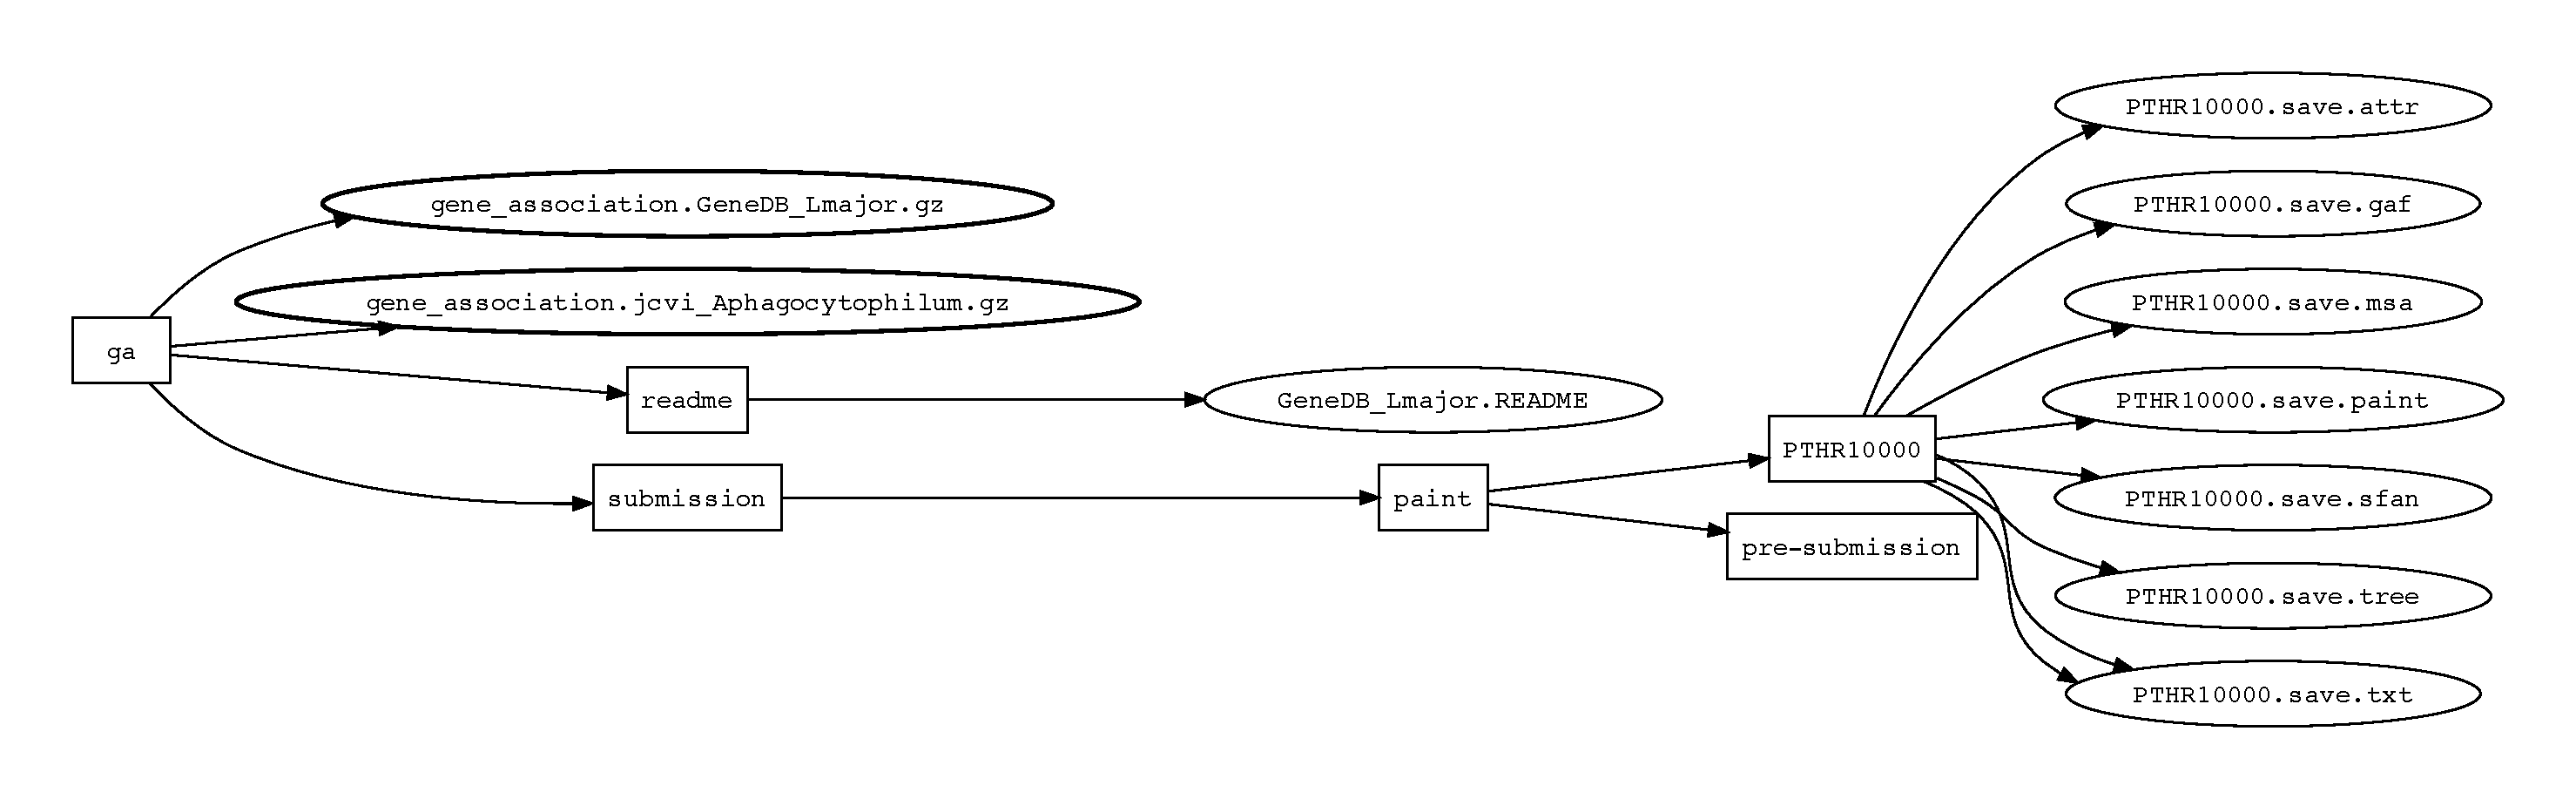
\includegraphics{ga.pdf}}
\end{center}
\caption{Graph showing structure of a small subset of the Gene Ontology \filestore, generated from 
  the description using \texttt{ForestGraph}}
\label{fig:ga}
\end{figure}


\newpage

\section{CVS.hs Description}

This section provides a generic description for CVS repositories.

\begin{code}
\textcolor{red}{-- PADS description of CVS file formats}
[pads| \kw{type} Repository_f = Line Pstringln

       \kw{data} Mode_t = Ext ":ext:" | Local ":local:" | Server ":server:" 

       \kw{data} Root_t = \{ cvs_mode :: Maybe Mode_t
                     , machine  :: Pstring ':', ':'
                     , path     :: Pstringln            
                     \}                                  
       \kw{type} Root_f = Line Root_t

       \kw{data} Dentry_t = \{ "D/"
                       , dirname :: Pstring '/'
                       , "////"
                       \}
\mbox{}
       \kw{data} Revision_t  = Version (Pint, '.', Pint) | Added '0' | Removed '-'
       \kw{data} TimeStamp_t = \{ ts       :: PstringSE (RE "[/+]")
                          , conflict :: Maybe ('+', Pstring '/') \}
\mbox{}
       \kw{type} Fentry_t = \{                                  "/"  
                       , filename   :: Pstring '/',       "/"
                       , revision   :: Revision_t,        "/"
                       , timestamp  :: TimeStamp_t,       "/"   
                       , options    :: Pstring '/',       "/"  
                       , tagdate    :: Pstringln
                       \}

       \kw{data} Entry_t   = Dir Dentry_t | File Fentry_t | NoDir 'D'
     
       \kw{type} Entries_f = [Line Entry_t] \kw{with} term Eof
|]
\end{code}
\begin{code}

\textcolor{red}{-- Auxiliary Haskell functions}
getEntries cvs = \kw{let} (Entries_f l) = entries cvs \kw{in} l
getDirName  d  = \kw{let} (Pstring s)   = dirname   d \kw{in} s
getFileName f  = \kw{let} (Pstring s)   = filename  f \kw{in} s
\mbox{}             
isDir entry  = \kw{case} entry \kw{of} {Dir _  -> True; otherwise -> False}
isFile entry = \kw{case} entry \kw{of} {File _ -> True; otherwise -> False}
\mbox{}                            

getDirs  cvs = map (\textbackslash(Dir d)  -> d) (filter isDir  (getEntries cvs))
getFiles cvs = map (\textbackslash(File f) -> f) (filter isFile (getEntries cvs))
\end{code}
\begin{code}

\textcolor{red}{-- FOREST description of CVS directory structure}
\textcolor{red}{-- Note that this description is recursive.}
\textcolor{red}{-- Note also that the collection of dirs and the 
-- collection of files are determined from information in the cvs 
-- directory.}
[forest| \kw{type} CVS_d = \kw{Directory}
              \{ repository \kw{is} "Repository" :: File Repository_f
              , root       \kw{is} "Root"       :: File Root_f
              , entries    \kw{is} "Entries"    :: File Entries_f
              \}
\mbox{}             
         \kw{type} CVS_Repository_d = Directory
             \{ cvs         \kw{is} "CVS"                 :: CVS_d
             , dirs        \kw{is} [ n \kw{as} <| getDirName  d |> :: CVS_Repository_d | d <- <| getDirs  cvs |> ]
             , files       \kw{is} [ <| getFileName f |> :: Text       | f <- <| getFiles cvs |> ]
             \} |]

\end{code}
\begin{code}
\textcolor{red}{-- Sample use of PADS and FOREST descriptions}
meta_dir     = "Examples/CVS"
entries_file = meta_dir ++ "/Entries"
doParseEntries = \kw{do} \{
 (rep, md)  <- parseFile entries_file
\}
\mbox{}             
doLoadCVS = \kw{do} \{
   (meta_rep, meta_md) <- cVS_d_load meta_dir
\}
\end{code}

\section{Universal.hs Description}

This section includes a universal data description.  This universal description
is used to drive some of our generic tools.

\begin{code}
\textcolor{red}{-- Universal Forest Directory Description}

[forest| 
  \kw{type} Universal_d = \kw{Directory}
     \{ ascii_files  \kw{is} [ f :: Text        | f <- \kw{matches} (GL "*"), <| get_kind  f_att == AsciiK     |> ]
     , binary_files \kw{is} [ b :: Binary      | b <- \kw{matches} (GL "*"), <| get_kind  b_att == BinaryK    |> ]
     , directories  \kw{is} [ d :: Universal_d | d <- \kw{matches} (GL "*"), <| get_kind  d_att == DirectoryK |> ]
     , symLinks     \kw{is} [ s :: SymLink     | s <- \kw{matches} (GL "*"), <| get_isSym s_att == True       |> ]
     \} 
|]
\end{code}
\begin{code}

\textcolor{red}{-- Use of Universal directory}
universal_dir = "Examples/data/universal"
doLoadUniverse = \kw{do} \{
 (rep, md) <-  universal_d_load  universal_dir
 \}
\end{code}


\end{document}



